\clearpage
\chapter{Beacon Tracking using ESP32 and Raspberry Pi.}
\section{Objective}
The UGV should move towards the maximum vicinity( on the basis of RSSI or Received Signal Strength Indicator  values) of beacon networks in an indoor environment in minimum time.

\section{Required components/Software tools}
\begin{itemize}
    \item Raspberry Pi (3B model) for main controller
    \item ESP32 micro-controller with Type-B USB cable
    \item L293D Motor Driver IC
    \item UGV chassis with DC motors
    \item Breadboard
    \item Jumper Wires
    \item Android phone used as beacon
\end{itemize}

\begin{figure}[h!]
\centering
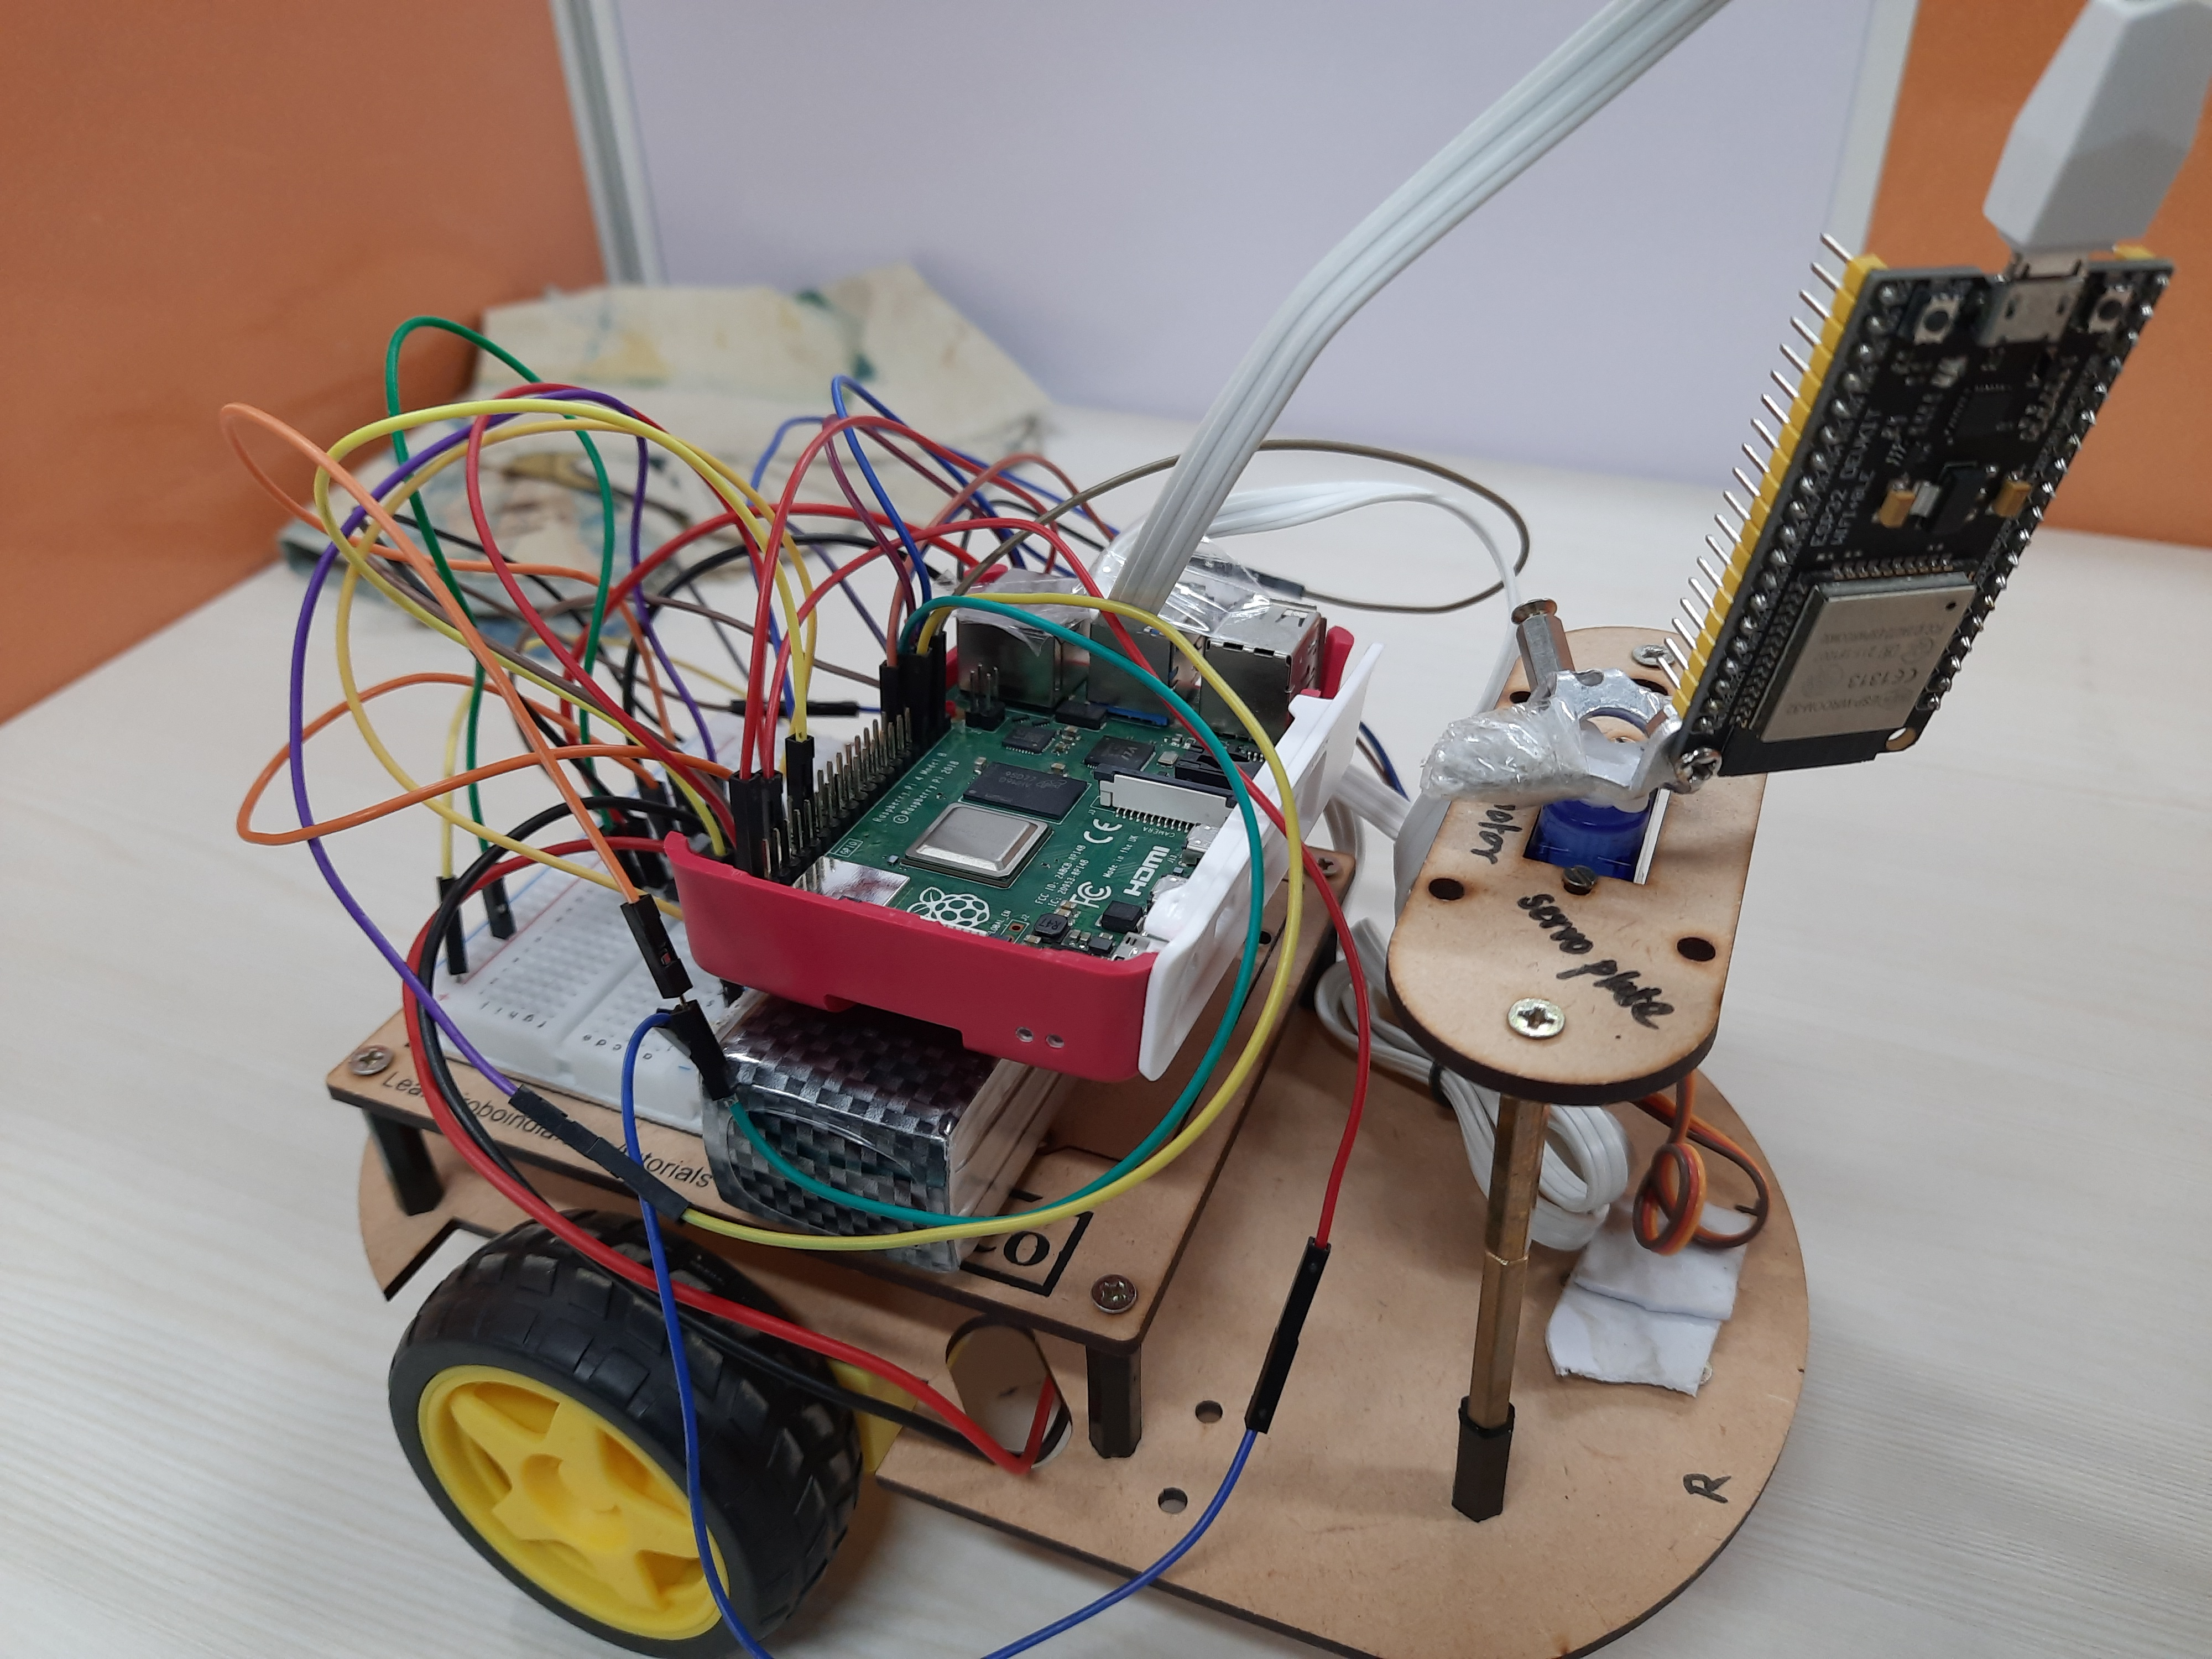
\includegraphics[width=10cm]{./Figures/beacon_tracking.jpg}
\caption{UGV kit assembly for beacon tracking}
\label{beacon_tracking}
\end{figure}

\begin{figure}[h!]
\centering
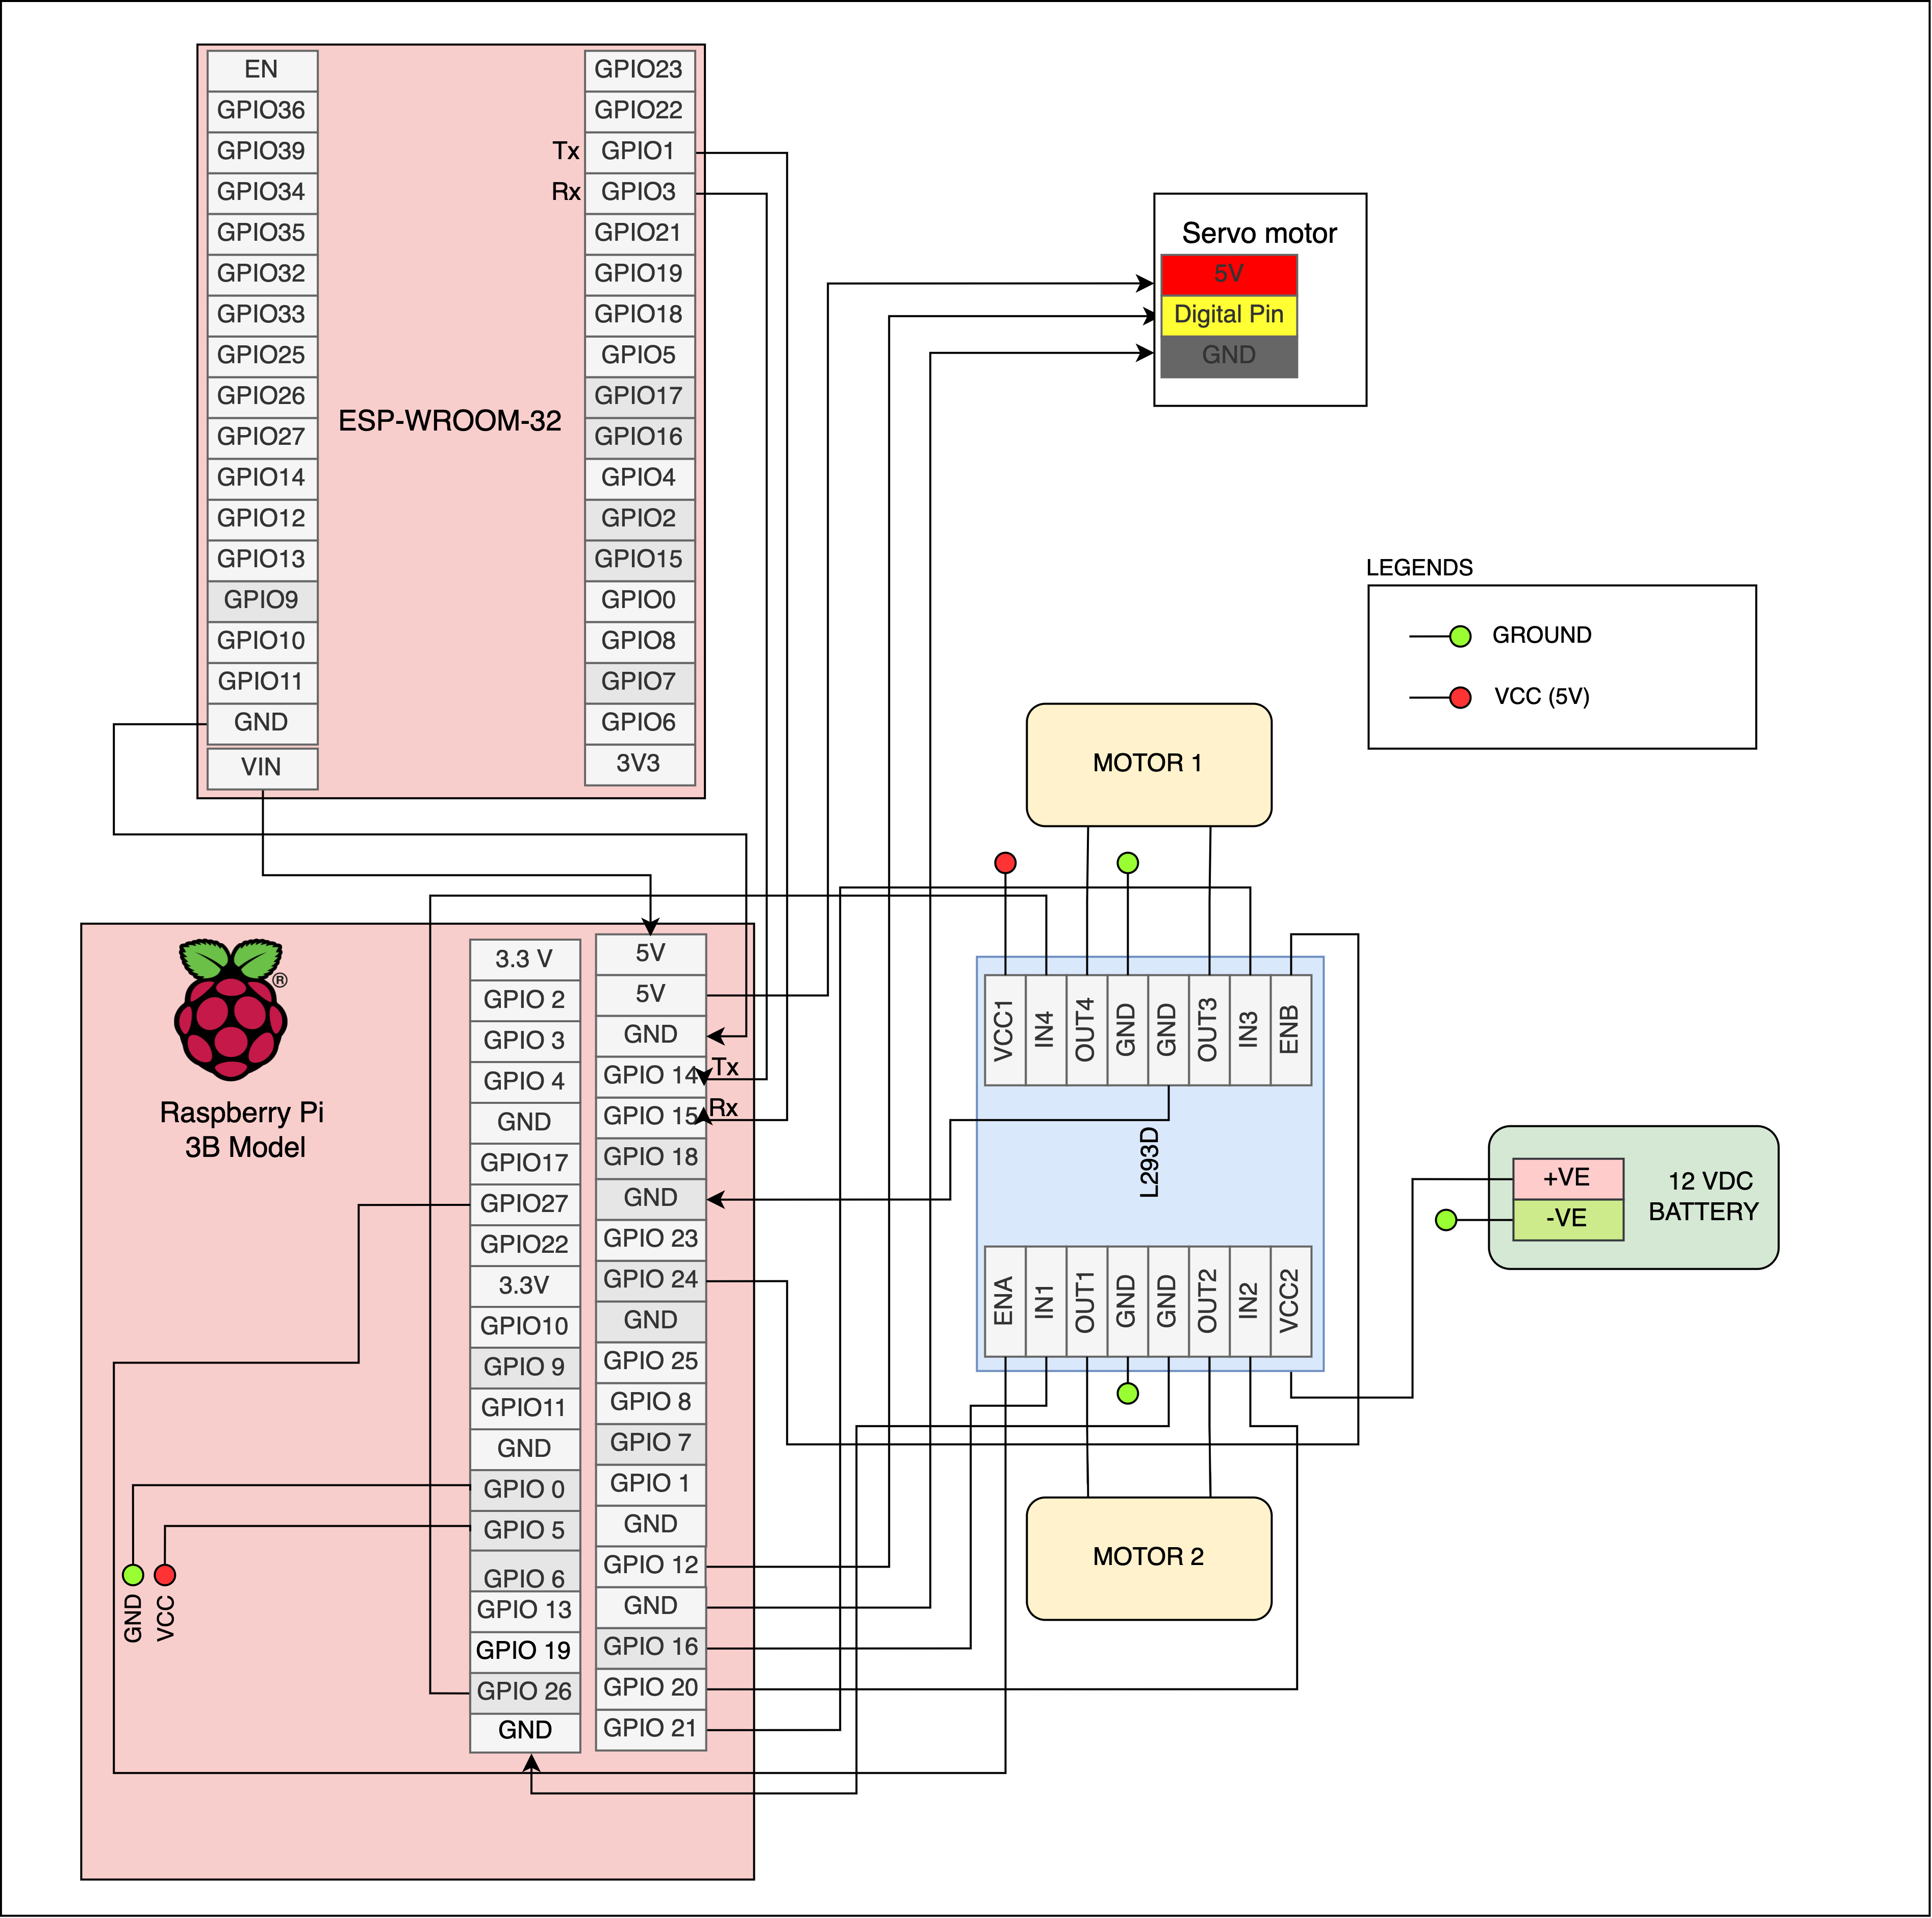
\includegraphics[width=\columnwidth]{./Figures/Wiring_beacon.png}
\caption{Wiring diagram for Beacon Tracking system (used in Method 2)}
\label{Wiring_beacon}
\end{figure}

\section{Methodology used:}
\subsection{Method 1:}
Initially, we tried the moving average method on RSSI values received by the ESP32 module.
\begin{itemize}
    \item Step 1: Initially, ESP32 mounted on the car will read RSSI (Received Signal Strength Indicator) levels in forward, right and left direction by suitable in-place rotation.
    
    \item Step 2: Average of 20 RSSI values are taken while measuring RSSI level in a particular direction. This is done in order to read stable RSSI values.
    
    \item Step 3: The car then rotates towards the direction having the highest RSSI level.
    \item Step 4: Further, It moves forward for a certain distance towards the beacon. By repeating the above steps again and again, the car navigates towards the beacon.
\end{itemize}
\textbf{Note:} Above method works but it takes more time to reach the beacon location. Hence, we moved towards the ML based algorithm i.e, KNN ( K- Nearest Neighbours).

\newpage
\subsection{Method 2: KNN algorithm (Machine Learning based method)}

\begin{itemize}
    \item \textbf{Step1:} Collection of data in the lab. Data has been collected in an indoor environment ( 14x10 square feet area) Each block area is around 2 feet. (Refer Figure \ref{angle_ref_beacon} and \ref{bot_angle_pos_beacon})
    
    \begin{figure}[h!]
    \centering
    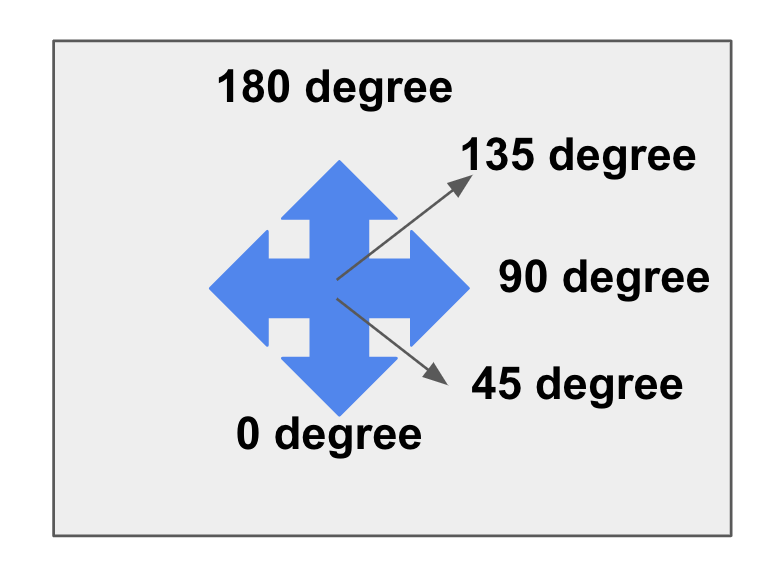
\includegraphics[width=8cm]{./Figures/angle_ref_beacon.png}    \caption{Angle reference from beacon on each block}
    \label{angle_ref_beacon}
    \end{figure}
    
    \begin{figure}[h!]
    \centering
    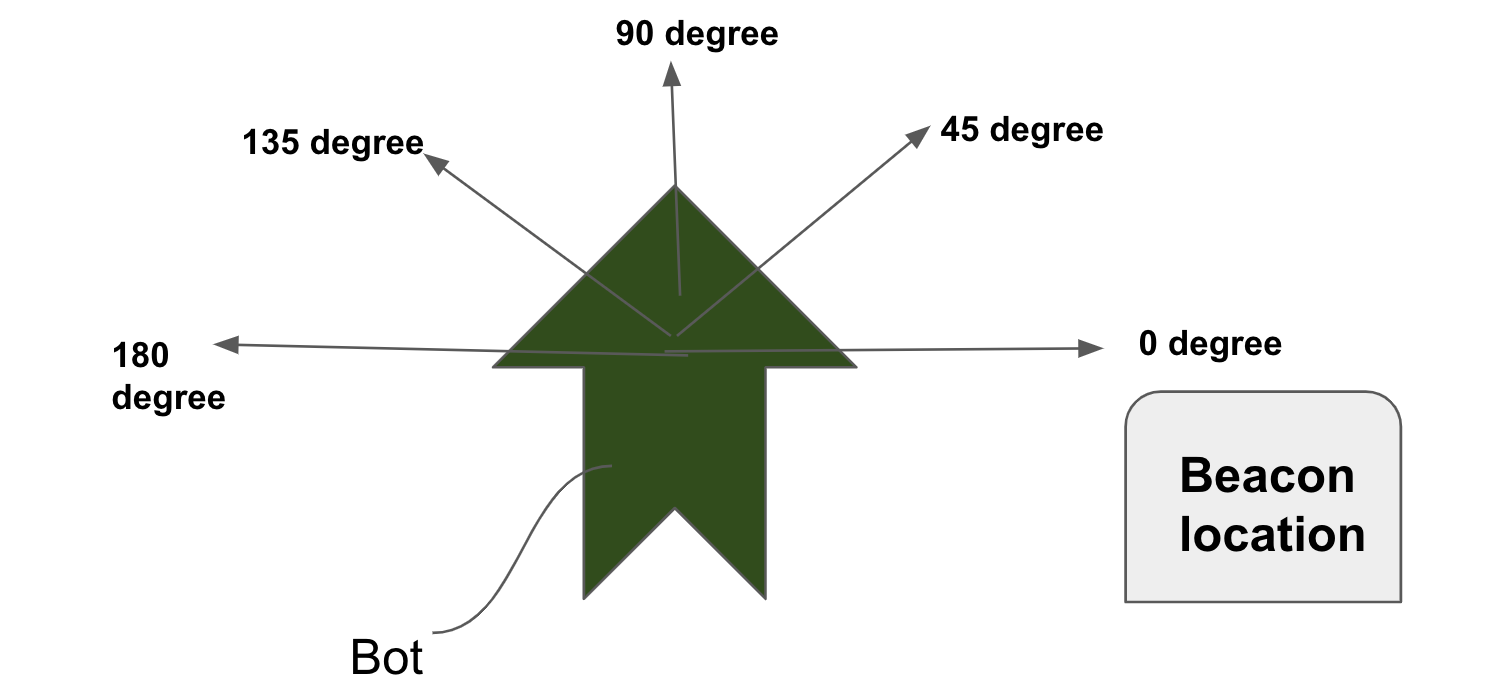
\includegraphics[width=12cm]{./Figures/bot_angle_pos_beacon.png}
    \caption{With reference to beacon, bot`s required angle positions are described.}
    \label{bot_angle_pos_beacon}
    \end{figure}
    
    \item \textbf{Step 2:} From each direction at each block ( refer fig.3) , 15 continuous RSSI values were received by ESP32 module and sent those real-time values to our local machine( laptop) in a spreadsheet(for storing purpose)  using raspberry pi. (Refer Figure \ref{beacon_tracking_arena})
    
    \begin{figure}[h!]
    \centering
    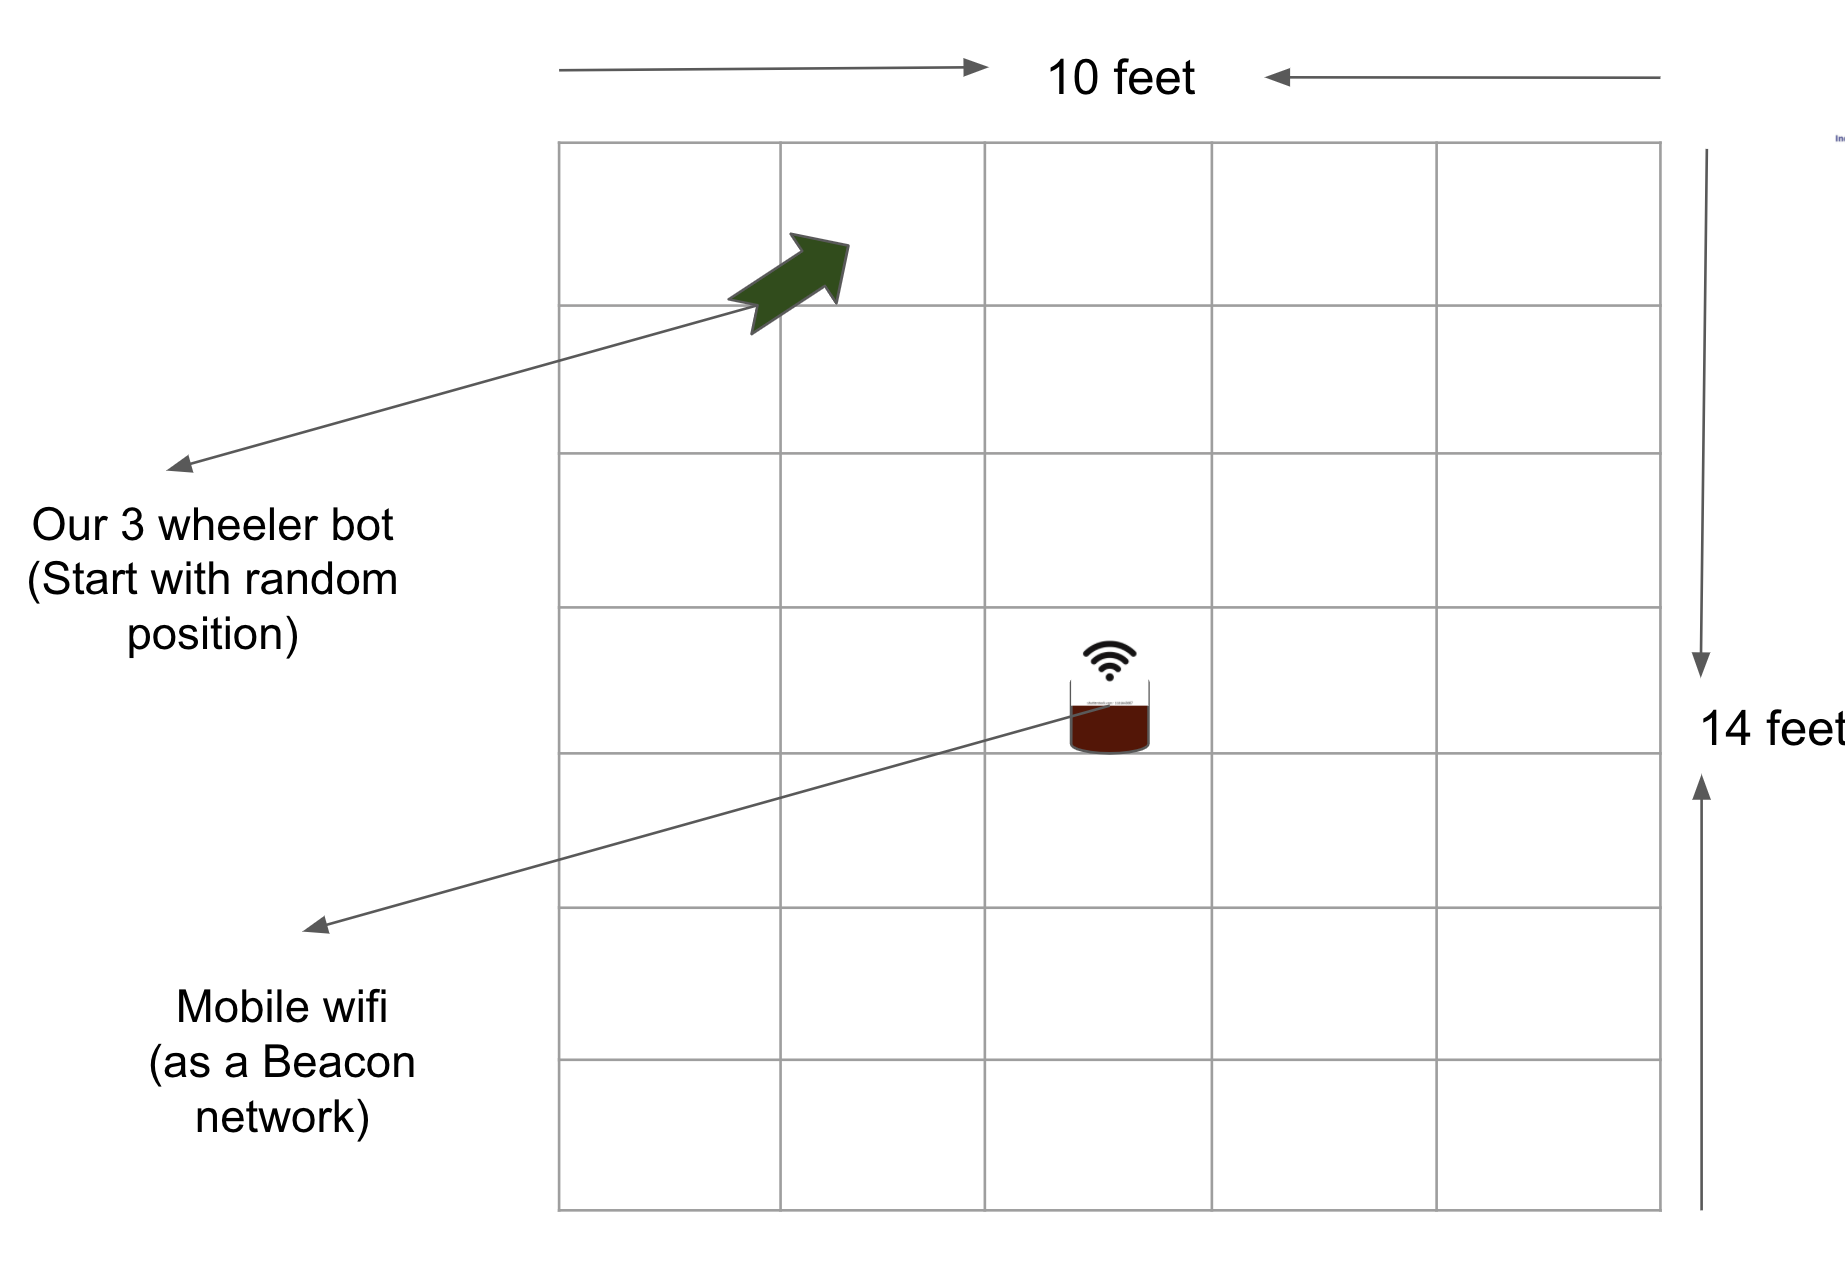
\includegraphics[width=\columnwidth]{./Figures/beacon_tracking_arena.png}
    \caption{Arena for data collection}
    \label{beacon_tracking_arena}
    \end{figure}
    
    \item \textbf{Step 3:} We had collected (2040 x 5) data-set containing RSSI values coming from beacon, received by ESP32 in 5 different directions (eg. 0, 45, 90, 135, 180 degree angles) in spreadsheet for future reference.(Refer figure \ref{beacon_data_snapshot})
    \item\textbf{ Step 4:} We manually put encoded angular direction values for true label (total 5 classes):
    \begin{itemize}
        \item 0 degree      : 0 
        \item 45 degree    : 1
        \item 90 degree    : 2
        \item 135 degree  : 3
        \item 180 degree  : 4
    \end{itemize}
    
    \begin{figure}[h!]
    \centering
    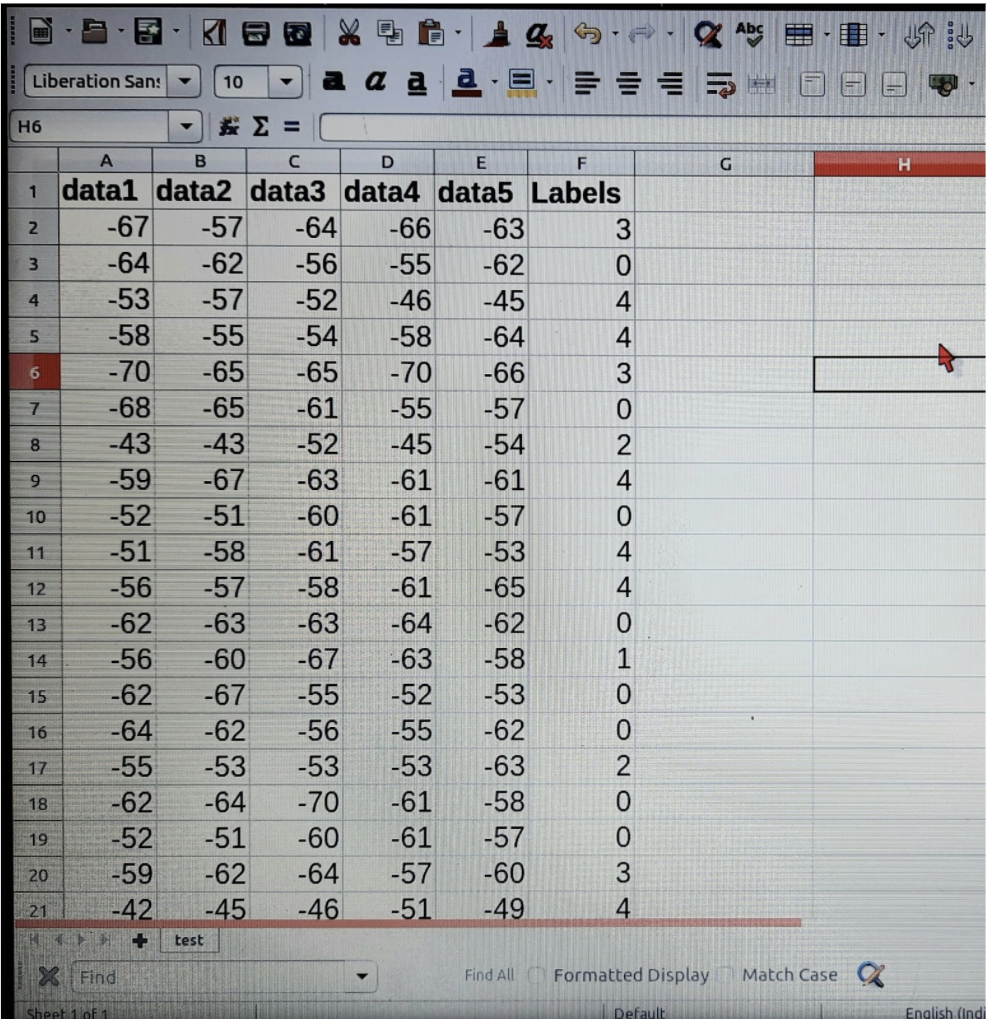
\includegraphics[width=10cm]{./Figures/beacon_data_snapshot.png}
    \caption{A snap of our collected RSSI data }
    \label{beacon_data_snapshot}
    \end{figure}
    
    \item \textbf{Step 5:} KNN Model training and testing 
    \begin{itemize}
        \item The K Nearest Neighbor algorithm comes under the Supervised Learning and is used for classification (most commonly) and regression also. 
        \item It considers K Nearest Neighbors (data points) to predict the class or continuous value for the new data-point.
        \item In KNN, we do not learn weights from training data to predict output (as we do in model-based algorithms) but use entire training instances to predict output for unseen data.
        \item Step 1: The data-set which we have prepared, is splitted into 80:20 ratio for train & test.
        \item Step 2: We have implemented the KNN algorithm on our data-set.
        \item Step 3: On new test data it gives approximately 77.08\%  accuracy ( used sklearn library in Google colaboratory for model training). 
    \end{itemize}
\end{itemize}
\textbf{Results and Conclusion:} Although we tried KNN in order to reduce the time taken by the whole process as we did in method 1, KNN did not give consistent results on new test data points. Hence, we came upon the conclusion that we should solve this beacon tracking problem using method 1 with time and accuracy trade-off.
\newpage
\subsection{Code and Data-set link}
\begin{tcolorbox}
        \url{https://github.com/Abhishek-IITH/Projects/tree/main/Beacon_tracking}
\end{tcolorbox}